\section{Banda della Maglia}\label{banda-della-maglia}

Tags: Organizzazione Creatore: Lorenzo Luogo: Sud Valtara

\section{Banda della Maglia}\label{banda-della-maglia-1}

\begin{center}\rule{0.5\linewidth}{0.5pt}\end{center}

\begin{center}\rule{0.5\linewidth}{0.5pt}\end{center}

\begin{figure}
\centering
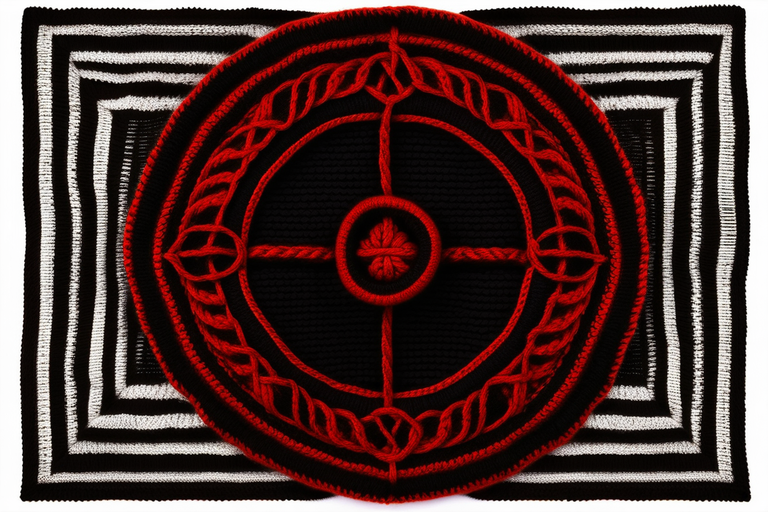
\includegraphics{black-symbol-with-red-wool-sweater-in-the-center_(1).png}
\caption{black-symbol-with-red-wool-sweater-in-the-center (1).png}
\end{figure}

Informazioni Generali

Tipo: Banda Criminale

Struttura:

Regione: Sud Valtara (Valtara)

Fondatore:

Membri:

Alleati:

Nemesi: Gilda dei Commercianti del Sud Valtara, Regno degli Alisei

\subsection{1. Descrizione Generale}\label{descrizione-generale}

\begin{center}\rule{0.5\linewidth}{0.5pt}\end{center}

La Banda della Maglia è un'organizzazione malavitosa attiva nella
regione della Valtara Meridionale, nota per le sue attività illegali nel
traffico di tessuti pregiati. La sua presenza è ben radicata nel
sottobosco criminale, spesso sfuggendo alla sorveglianza delle forze
dell'ordine grazie alla sua rete di complici e alle tattiche di
infiltrazione raffinate. La banda è conosciuta per la sua abilità nel
manipolare il mercato tessile e nel controllare le forniture di
materiali pregiati, garantendo il proprio potere e influenza nelle
industrie tessili locali.

\subsection{2. Storia}\label{storia}

\begin{center}\rule{0.5\linewidth}{0.5pt}\end{center}

La Banda della Maglia è nata in momento di crisi della Gilda dei
Commercianti del Sud Valtara, dovuta ad un periodo di instabilità
politica e conseguente crisi economica nel regno degli Alisei. Con i
prezzi dei tessuti in costante aumento e le restrizioni imposte dal
regno, la domanda di materiali tessili è cresciuta in modo esponenziale.
Sfruttato questo scenario, la Banda ha iniziato a infiltrarsi nei
circuiti di approvvigionamento della Gilda, aprendo tratte commerciali
alternative e garantendo un flusso costante di tessuti sul mercato nero.
In poco tempo la banda è riuscita a mantenere un controllo saldo sul
commercio illegale di tessuti, guadagnando notevoli profitti anche dopo
la fine del periodo di crisi economica. La Banda della Maglia si trova
costantemente nel mirino sia della Gilda dei Commercianti del Sud
Valtara che del regno degli Alisei, che hanno iniziato a intensificare
le loro azioni per neutralizzare la minaccia rappresentata
dall'organizzazione. La taglia posta sulle teste dei capi della Banda è
cospicua, attirando cacciatori di taglie e avventurieri desiderosi di
ottenere ricompense sostanziose. Gli arresti, seppur numerosi ogni anno,
colpiscono spesso solo i pesci piccoli dell'organizzazione, poiché i
leader stessi sono dotati di reti di protezione e di una rete di
contatti estesa e ben posizionata all'interno delle sfere politiche e
commerciali.

\subsection{3. Valori}\label{valori}

\begin{center}\rule{0.5\linewidth}{0.5pt}\end{center}

I membri dell'organizzazione sono noti per le loro tattiche spietate, e
non esitano a ricorrere alla violenza e all'intimidazione per ottenere
ciò che desiderano. La loro priorità principale è generare profitti, e
non esitano a infrangere la legge per raggiungere questo obiettivo.
L'avidità e l'egoismo dominano la loro filosofia, e la Banda è disposta
a tutto pur di accrescere la propria ricchezza e il proprio potere.

\subsection{4. Attività}\label{attivituxe0}

\begin{center}\rule{0.5\linewidth}{0.5pt}\end{center}

La Banda della Maglia non esita a impiegare metodi coercitivi e violenti
per costringere i produttori di tessuti a destinare una parte
consistente delle loro merci al mercato nero. Talvolta, le azioni della
Banda hanno portato a scontri violenti all'interno della comunità dei
produttori, minacciando l'integrità stessa del settore tessile locale.
Inoltre, la Banda controlla diverse fabbriche segrete, in cui produce
falsi di alta qualità che vengono immetti nel mercato legale come
autentici. Queste attività illegali hanno consolidato ulteriormente la
loro influenza all'interno del mercato tessile, creando un'aura di sfida
e pericolo intorno alla Banda della Maglia che ha spinto molti a cercare
alleanze con loro, temendo di diventarne vittima.
